\chapter{Expunerea tehnologiei}

\section{Serviciul NLU}
Urmărind scopul practic al acestei lucrări se conturează nevoia de a avea tehnologia de NLU expusă la nivel de serviciu web.
În concordanță cu paradigma de SaaS (software as a service) am mai dezvoltat încă un strat de abstractizare peste modelul de NLU (figura \ref{fig:nlu_arch}).
Serverul este scris cu ajutorul frameworkului de dezvoltare web, flask. Cu ajutorul său implementarea modelului de NLU este expusa în rețea sub forma unei resurse web ce poate fi interogată trimițând textul dorit.
Răspunsul serviciului (anexa \ref{lst:rsp}) este unul detaliat ce ne oferă și încrederea cu care modelul a prezis.
\begin{figure}[h]
	\centering
	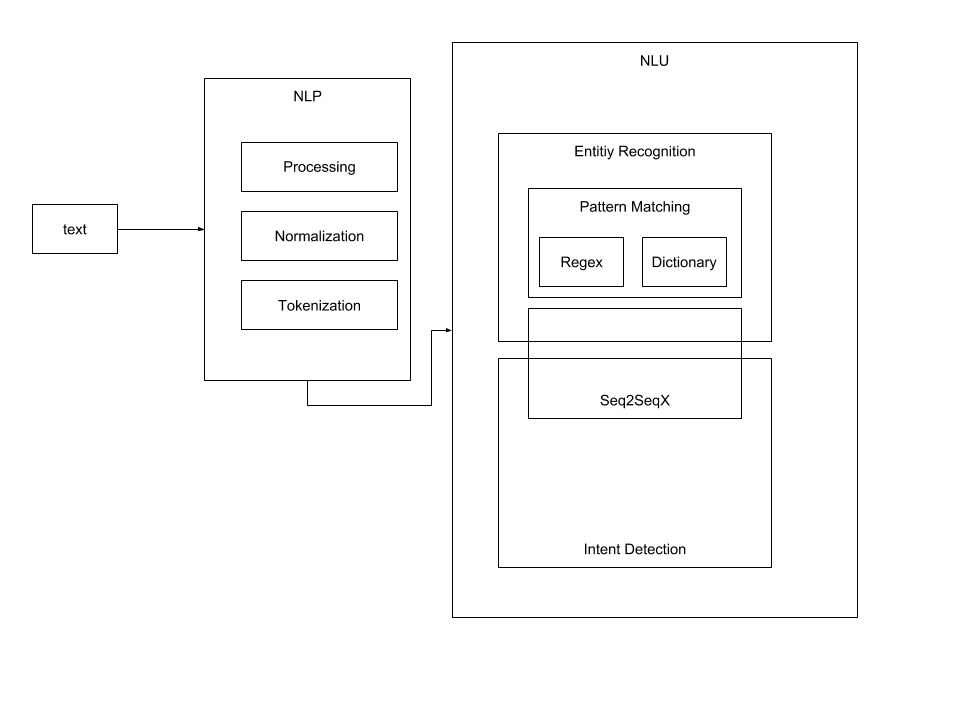
\includegraphics[scale=0.4]{nlu_architecture.png}
	\caption{Arhitectura serviciului de NLU}
	\label{fig:nlu_arch}
\end{figure}

\section{Tehnologii folosite}

Desemnarea tehnologiilor open source folosite ca dependențe poate fi văzută la prima vedere o alegere ușoară, însă este nevoie de o analiză mult mai amănunțită în ceea ce privește specificul proiectului.
Pentru această lucrare am luat în considerare următorii factori: complexitatea de a descrie o rețea neuronală, modul de expunere (la nivel de API) al proceselor matematice din spate și flexibilitatea de a putea jongla cu diferite arhitecturi de rețele. De asemenea eficiența și posibilitatea de a rula pe diferite unități de calcul (CPU/GPU).

\subsection{Python}

Limbajul de programare utilizat în implementarea modelelor propuse este Python. El este folosit de la dezvoltare de servicii web (django, flask) până la biblioteci software de învățare automată (pytorch, tensorflow). Datorită popularității sale el se bucură din plin de licențierea open source, având o comunitate impresionantă de oameni care contribuie la dezvoltarea acestui ecosistem, cel puțin în partea de inteligență artificială el este instrumentul cel mai folosit și are cele mai multe pachete care îi extind funcționalitatea. 

Python a fost creat la începutul anilor 1990 de Guido van Rossum la Stichting Mathematisch Centrum (CWI) în Olanda ca un succesor al limbajului ABC. \cite{pythonhistory}. Este un limbaj orientat pe obiecte ce vine însoțit de structuri de date la nivel înalt (dicționare, mulțimi, liste), uneori împrumutând concepte din programarea funcțională (list comprehention, map/reduce), alteori din programarea paralelă (apeluri asincrone).

\subsection{Numpy}

Pentru lucrul cu matrice și alte structuri ce impun operații algebrice vectoriale se folosește de obicei Numpy. El este un acronim pentru "Numeric Python" sau "Numerical Python". Este un pachet fundamental pentru calculul științific in Python, ce furnizează funcții precompilate care se execută rapid cu scopul de a efectua operațiile matematice de rutină.

\subsection{PyTorch}

PyTorch \cite{pytorch} este o bibliotecă software ce oferă un cadru de lucru cu algoritmi de învățare automată. Se prezintă ca o variantă de Numpy care poate rula pe placa video, având totodată și capacitatea de autodiferențiere atunci când este nevoie să antrenăm, spre exemplu folosind metoda gradientului descendent.

\textbf{Diferențiere Automată}

Componenta cheie a rețelelor neuronale din PyTorch este pachetul \textit{autograd}. El oferă diferențierea automată pentru toate operațiile cu \textit{tensori}. Este un cadru de definire a operațiilor (forward dar și backward) la momentul execuției, ceea ce înseamnă că pasul de backpropagation este definit de modul în care este rulat codul.

\textbf{Tensor}

\textit{torch.Tensor} este clasa centrală a pachetului. Dacă se setează atributul \texttt{.requires\_grad} ca  \texttt{True}, se va începe urmărirea tuturor operațiilor în care acesta intervine. După ce se termină calculul, se poate apela \texttt{ backward()} pentru a calcula automat toate derivatele, iar gradientul pentru acest tensor va fi acumulat în atributul \texttt{.grad}.

Pentru a opri tensorul din istoricul de urmărire, se apelează \texttt{.detach()} care detașează tensorul de istoricul de calcul și care împiedica urmărirea viitoarelor calcule.

Mai există încă o clasă care este foarte importantă pentru implementarea autodiferențierii - și anume \textit{Function}.

Tensorul și funcția sunt interconectate și construiesc un graf aciclic, care codifică un istoric complet al calculelor. Fiecare tensor are un atribut  \texttt{.grad\_fn} care se referă la o funcție care a creat tensorul (cu excepția tensorurilor creați de utilizator unde - \texttt{.grad\_fn = None}).